\chapter{Overall Concept of the Developed Solutions}

% In this first result chapter of the thesis the overall concept which clarifies the relationship of the investigated issues is introduced.
% From this overall concept all further result chapters and the solutions covered by each of these chapters should be derived.

\section{Monitoring BestRental}

\subsection{Monitoring Targets}

Figure \ref{fig:sps_architecture_bestrental} shows the System Plus Software Architecture of the Demonstrator BestRental.

\begin{figure}
	\centering
	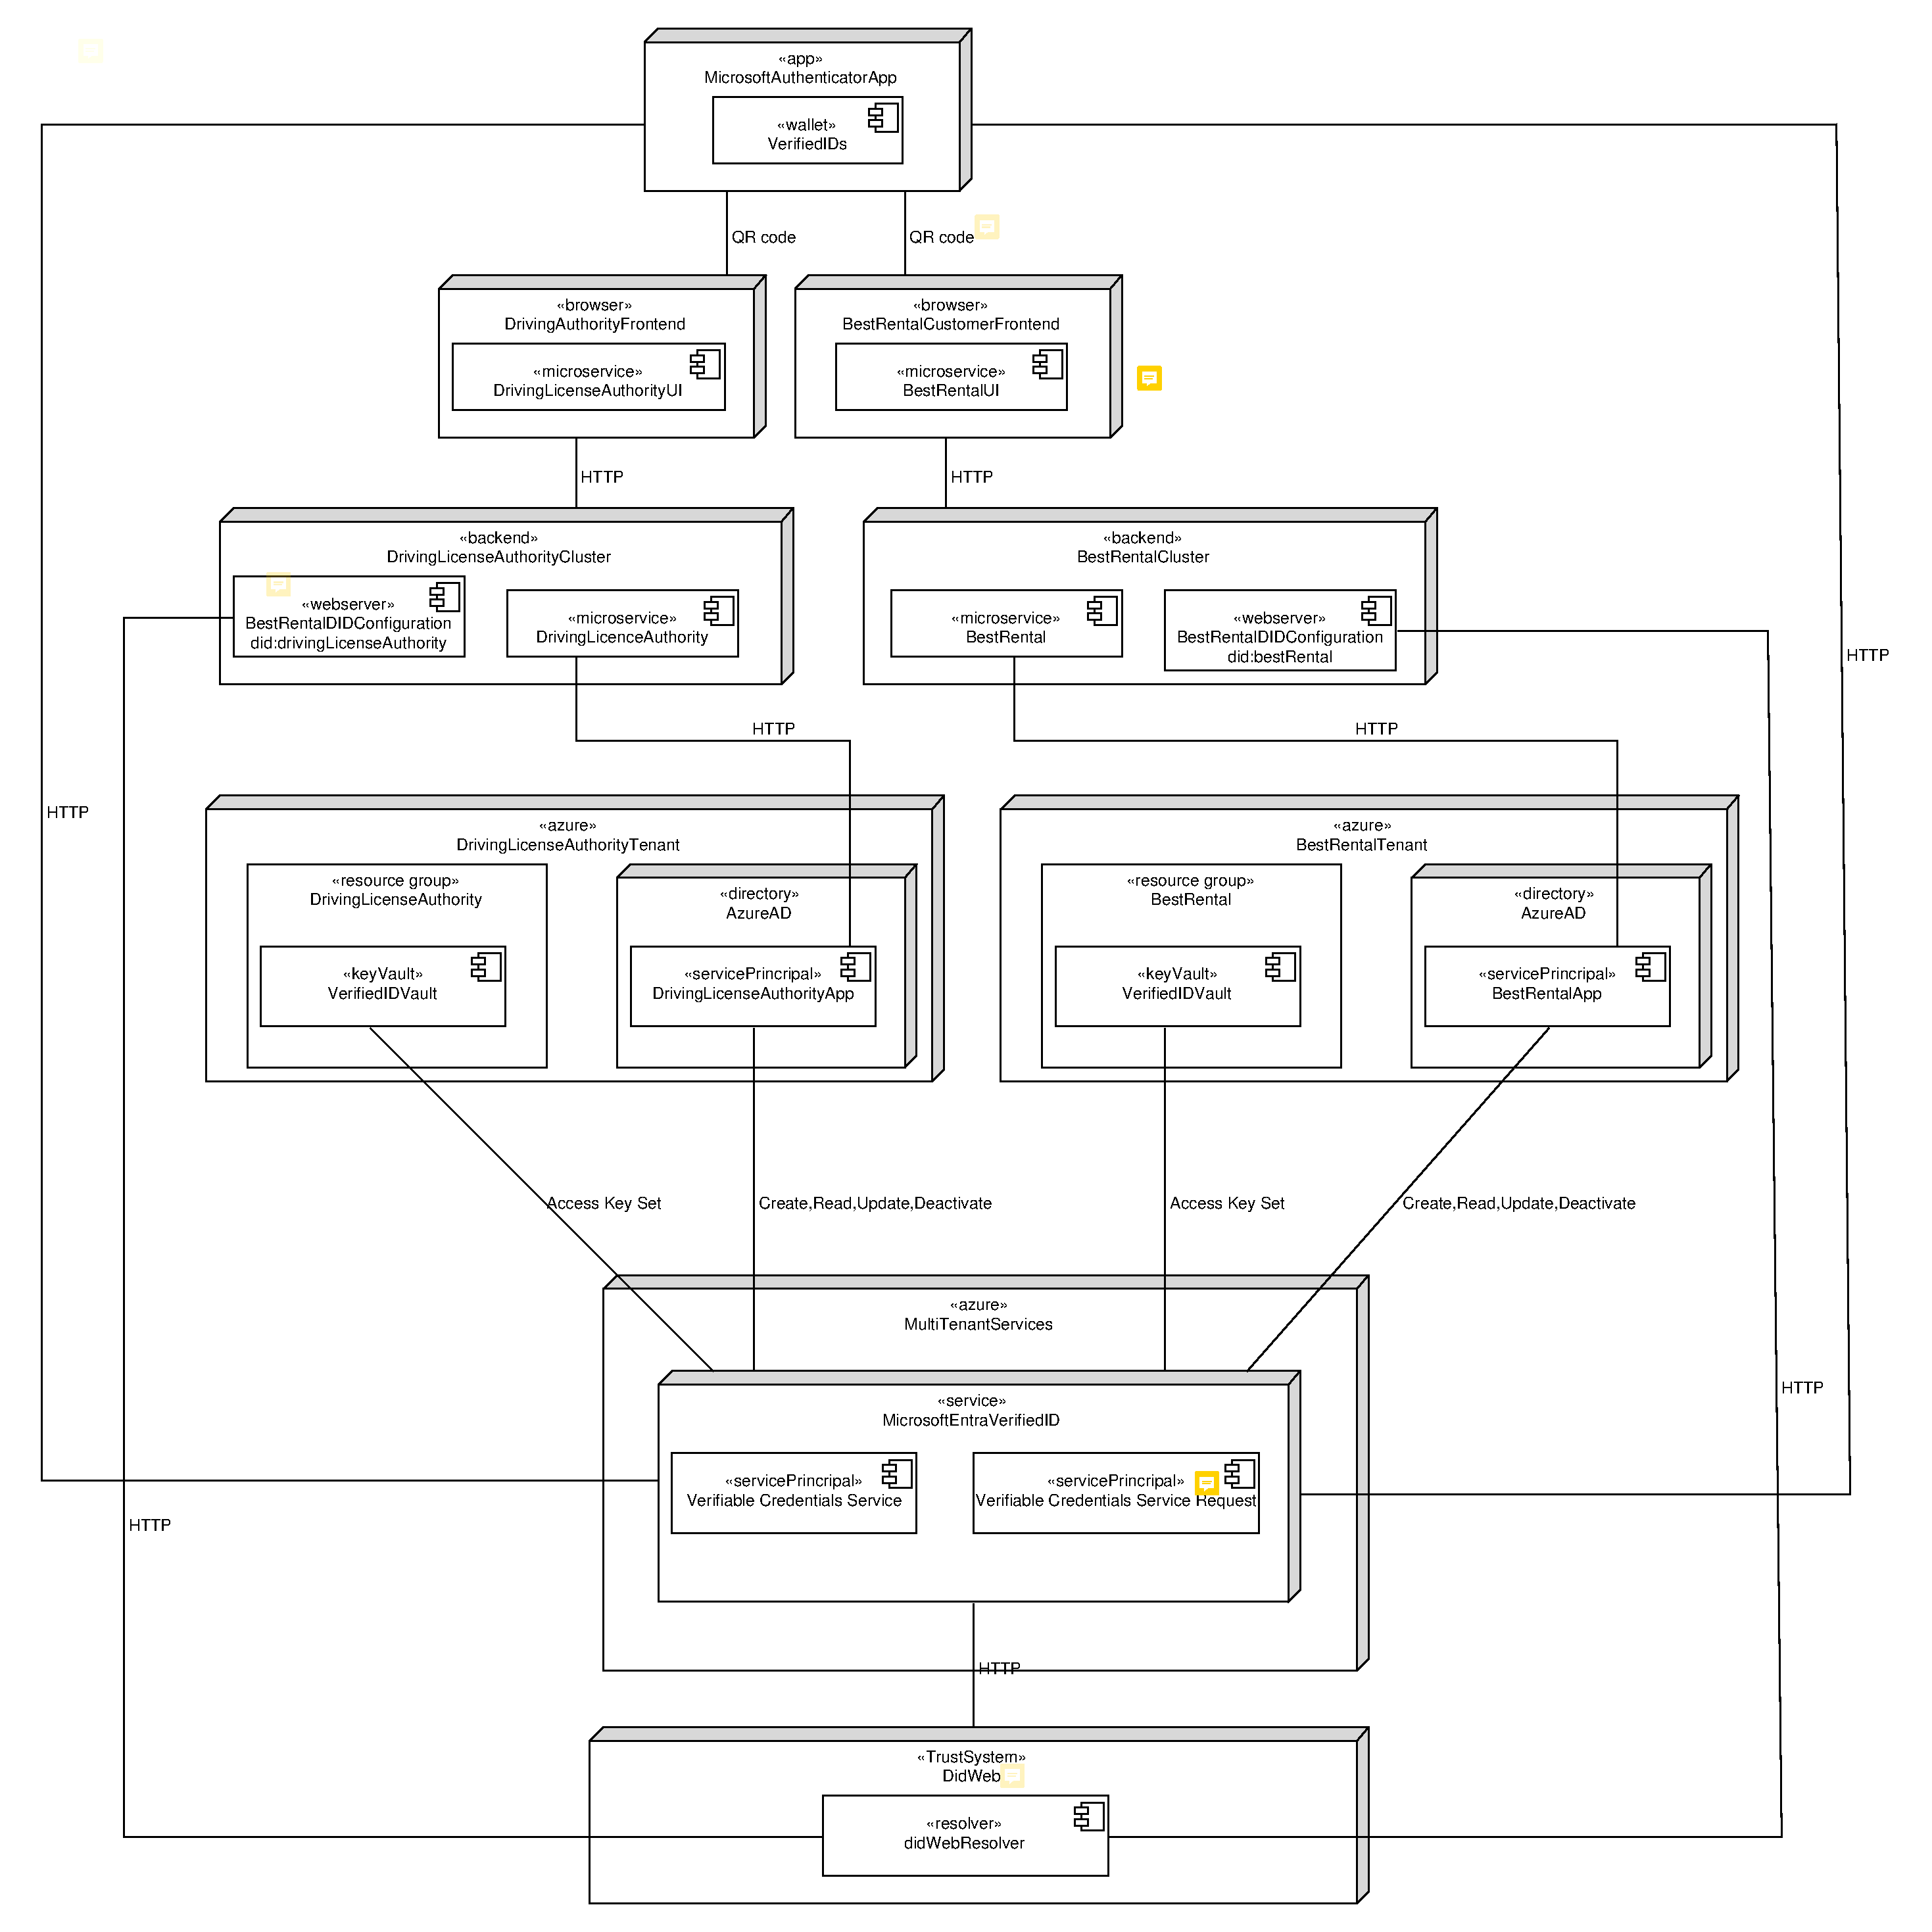
\includegraphics[width=\textwidth]{pdfs/sps_achitecture_bestrental.pdf}
	\caption{SystemPlusSoftware Architecture BestRental}
	\label{fig:sps_architecture_bestrental}
\end{figure}

The Demonstrator for BestRental includes multiple types of resources.
These can be grouped into internal and external resources.
\begin{enumerate}
    \item Microsoft Application: External
    \item Service: Internal
    \item Cluster: Internal
    \item Azure Tenant: External
    \item Azure Resource Group: External
    \item Azure Directory: External
    \item Service (Principal): External
    \item Trust System: External
    \item Trust Resolver: External
\end{enumerate}

For the collection of metrics from external Microsoft Azure resources, the service Azure Monitor can be used.
This service allows the export and import through a REST API.

\begin{table}[]
\begin{tabular}{ll}
   & Requirement       \\
R1 & High Availability \\
R2 & Scalability       \\
R3 & Extensibility    
\end{tabular}
\caption{Requirements for a Monitoring Solution}
\label{tab:requirements}
\end{table}

\begin{table}[]
\begin{tabular}{ll}
     & Objective                                   \\
QoS1 & Application uptime                          \\
QoS2 & Maximum latency                             \\
\end{tabular}
\caption{Quality of Service Objectives}
\label{tab:qos_objectives}
\end{table}

\begin{table}[]
\begin{tabular}{llll}
    & Metric                                             & Motivation                       & Internal/External resources/Application \\
M01 & Active Sessions                                    & Performance Management           & Application                             \\
M02 & Login attempts                                     & Security Management              & Application                             \\
M03 & Average failed login attempts per session          & Security Management              & Application                             \\
M04 & Maximum failed login attempts per session          & Security Management              & Application                             \\
M05 & Total incoming requests per hour                   & Performance Management           & Application                             \\
M06 & Average incoming requests per session per hour     & Performance Management           & Application                             \\
M07 & Average incoming requests per service per hour     & Performance Management           & Internal                                \\
M08 & Average outgoing requests per service per hour     & Performance Management           & Internal                                \\
M09 & Total failed requests                              & SLA Management                   & Application                             \\
M10 & Total failed requests per service                  & Troubleshooting                  & Internal/External                       \\
M11 & Average failed requests per session                & SLA Management                   & Application                             \\
M12 & Average latency for incoming requests              & SLA Management                   & Application                             \\
M13 & Average latency between services                   & Performance Management           & Internal                                \\
M14 & Maximum resource usage of service                  & Capacity and Resource Management & Internal                                \\
M15 & Average resource usage of service in the last hour & Capacity and Resource Management & Internal                                \\
M16 & Total accumulated cost                             & Billing                          & Application                             \\
M17 & Accumulated cost per service                       & Billing                          & Internal/External                       \\
M18 & Total application downtime                         & SLA Management                   & Application                             \\
M19 & Downtime per service                               & SLA Management                   & Internal/External                      
\end{tabular}
\caption{Monitoring Metrics}
\label{tab:monitoring_metrics}
\end{table}